% Created 2023-09-11 Mon 08:14
% Intended LaTeX compiler: pdflatex
\documentclass[11pt]{article}
\usepackage[utf8]{inputenc}
\usepackage[T1]{fontenc}
\usepackage{graphicx}
\usepackage{longtable}
\usepackage{wrapfig}
\usepackage{rotating}
\usepackage[normalem]{ulem}
\usepackage{amsmath}
\usepackage{amssymb}
\usepackage{capt-of}
\usepackage{hyperref}
\usepackage{minted}
\usepackage[a4paper]{geometry}
\usepackage{mathtools}
\author{Alexander Huss}
\date{\today}
\title{Parton Showers}
\hypersetup{
 pdfauthor={Alexander Huss},
 pdftitle={Parton Showers},
 pdfkeywords={},
 pdfsubject={},
 pdfcreator={Emacs 29.1 (Org mode 9.7)}, 
 pdflang={English}}
\begin{document}

\maketitle
\tableofcontents



\section{Introduction}
\label{sec:orga4f8c72}
We will investigate the gluon-emission probability off quarks and gluons and use that to implement a \textbf{very} simplified parton shower (single final-state leg, only primary branching, leading double-log, only \(k_T\) and not proper kinematics, \ldots{}).

\section{Emission probability and the Sudakov form factor}
\label{sec:org41a89c8}
In the leading double-log approximation (soft \emph{and} collinear emission), we have seen in the lecture that the emission probability is given as
\begin{align}
  \mathrm{d}\omega_{X\to X+g}
  &=
  \frac{2\alpha_s C_X}{\pi} \; \frac{\mathrm{d}\theta}{\theta} \; \frac{\mathrm{d}E}{E}
  \,,
\end{align}
where \(E\) denotes the energy of the emitted gluon and \(\theta\) the angle w.r.t. the parent particle.
We denote the emitting particle by ``\(X\)'' and \(C_X\) is the associated colour factor.
For quarks, \(C_X=C_F=\tfrac{4}{3}\) and for gluons \(C_X=C_A=3\).

For any parton shower, we need to choose an evolution variable w.r.t. which we want to generate ordered emissions (angle \(\theta\), transverse momentum \(k_T\), virtuality \(q^2\), \ldots{}).
We will perform a slight change of variables, \(k_T \propto E \theta\) (transverse momentum w.r.t. the parent parton) and \(z \propto E\) (energy fraction of the emitted gluon) and integrate out the momentum fraction with the \(k_T\) constraint to obtain the emission probability
\begin{align}
  \mathrm{d}\mathcal{P}_\text{emit}
  &=
  \frac{2\alpha_s C_X}{\pi} \; \frac{\mathrm{d}k_T}{k_T} \int_{k_T/k_T^\mathrm{max}}^1 \frac{\mathrm{d}z}{z}
  =
  \frac{2\alpha_s C_X}{\pi} \; \frac{\mathrm{d}k_T}{k_T} \ln\biggl(\frac{k_T^\mathrm{max}}{k_T}\biggr)
  \,,
\end{align}
where \(k_T^\mathrm{max}\) denotes the upper bound on the transverse momentum that the emission can carry and is of the order of the hard scale.

We will further integrate over \(k_T\) with a lower cut-off \(k_T^\mathrm{cut}\), below which we consider the emission to be unresolved, and get for the probability of a single resolved emission
\begin{align}
  \mathcal{P}_\text{emit}(k_T>k_T^\mathrm{cut})
  &=
  \frac{\alpha_s C_X}{\pi} \; \ln^2\biggl(\frac{k_T^\mathrm{max}}{k_T^\mathrm{cut}}\biggr)
  \,.
\end{align}
Note that this fixed-order result comes with a serious problem: For a power of \(\alpha_s\), we get two powers of a potentially large logarithm (the so-called ``double logarithms'' that appear frequently in higher-order calculations), a pattern that will continue to higher orders.
For some representative values (\(\alpha_s \sim 0.1\), \(k_T^\mathrm{cut} \sim \Lambda_\mathrm{QCD} \sim 0.2\,\mathrm{GeV}\), \(k_T^\mathrm{max} \sim 100\,\mathrm{GeV}\)), we quickly realize that the large logarithm compensates the small value of the coupling, giving rise to a non-converging expansion.
In such situations, where we are sensitive to large logarithms, we need to re-arrange the perturbative expansion in such a way to ``re-sum'' these large logarithms to all orders.

To accomplish this, we define the so-called Sudakov form factor \(\Delta(t,t')\), which is the probability for \emph{no resolved emissions} to happen between the evolution \(t \to t'\), where we introduced an ``evolution time'' \(t\equiv\ln(k_T^\mathrm{max}/k_T)\).
The Sudakov form factor is \emph{multiplicative}, i.e. obeys \(\Delta(t,t'') = \Delta(t,t') \Delta(t',t'')\), and satisfies a differential equation reminiscent of that of radiative decay (\(\mathcal{P_\text{no-emit}} = 1-\mathcal{P_\text{emit}}\)):
\begin{align}
\label{eq:Dsud}
  \frac{\mathrm{d}\Delta(t_0,t)}{\mathrm{d}t}
  &=
  \Delta(t,t') \; \frac{\mathrm{d}\mathcal{P_\text{no-emit}}}{\mathrm{d}t'}
  =
  - \Delta(t,t') \; \frac{\mathrm{d}\mathcal{P_\text{emit}}}{\mathrm{d}t'}
  \,,
\end{align}
which has a simple solution
\begin{align}
\label{eq:sud}
  \Delta(t,t')
  &=
  \Delta(t') / \Delta(t)
  \,,\nonumber\\
  \Delta(t)
  &\equiv \Delta(0,t)
  =
  \exp\biggl\{-\frac{\alpha_s C_X}{2\pi} \, t^2 \biggr\}
  =
  \exp\biggl\{-\frac{\alpha_s C_X}{2\pi} \, \ln^2\biggl(\frac{k_T^\mathrm{max}}{k_T}\biggr) \biggr\}
  \,,
\end{align}
which now has the large logarithm in the exponent.
This solution therefore accomplishes exactly what we wanted: sum up the problematic logarithms to all orders, and in doing so, tame the otherwise divergent behaviour (\(k_T\to0\)).
It turns out that we can use the Sudakov form factor to sample successive emissions (it is a Markovian process), which we discuss in the next section together with a simple implementation.

\section{Implementation}
\label{sec:org81c8626}

\subsection{Interlude: Sampling}
\label{sec:org761538f}
Assume we have a uniform random number generator at our disposal sampling values in the range \(r\in[0,1]\).
We wish to generate samples \(x_i\) drawn from a probability distribution \(p(x)\).
In the so-called \emph{inversion method}, we use the fact that the \emph{cumulant} distribution, \(P(x) = \int_{-\infty}^x\mathrm{d}x' p(x')\), is a strictly monotonic function with values in \(P(x)\in[0,1]\) (it is a probability).
We can thus obtain a sample \(x_i\) by drawing \(r_i\) uniformly from \([0,1]\) and then \emph{inverting} the relation \(r_i = P(x_i)\) for x\textsubscript{i}.
The sample \(x_i\) generated this way, follows the probability distribution \(p(x)\).

Often times, the cumulant of the distribution is not easy to invert.
In such cases, one can also use the \emph{rejection method} (or ``hit-and-miss'') by finding a simpler distribution \(\tilde{p}(x)\) that bounds \(p(x)\) from above (in the simplest case the bound is just a constant).
If we can draw samples from \(\tilde{p}(x)\), all we need to do is to correct for the difference with respect to \(p(x)\).
This can be accomplished by drawing another uniform random number \(s_i\in[0,1]\) and only accepting the point \(\tilde{x}_i\) generated with \(\tilde{p}(x)\) with the probability \(p(\tilde{x}_i)/\tilde{p}(\tilde{x}_i)\).


\subsection{Our Toy Shower}
\label{sec:org5c66956}
With the Sudakov form factor in Eq. \eqref{eq:sud} at hand, we can easily iterate the sampling of emissions using the \emph{inversion method} described above given that the cumulant that corresponds to the probability for the \emph{next emission} is precisely the Sudakov.
The steps of the shower are:
\begin{enumerate}
\item set \(k_T = k_T^\mathrm{max}\)
\item draw a uniform random number \(r\) in the range \([0,\,1]\)
\item solve \(r = \Delta(k_T, k_T')\) for \(k_T'\), which is the new emission scale.
\item if \(k_T'<k_T^\mathrm{cut}\), no resolvable emission can be generated:
Terminate loop.
\item ``generate'' the emission at \(k_T'\), set \(k_T = k_T'\) and go back to step 2.
\end{enumerate}
The shower cut-off \(k_T^\mathrm{cut}\) is typically set to \(\mathcal{1\,\mathrm{GeV}}\) and represents the scale at which the perturbative shower description breaks down and the generated emissions are handed over to the hadronization model to simulate the non-perturbative hadronization stage of the simulation.

\begin{minted}[frame=lines,fontsize=\scriptsize]{python}
#!/usr/bin/env python

import math
import random
import sys
import numpy as np

random.seed(42)
alphas = 0.118


def generate_emissions(kt_max: float, kt_cut: float, CX: float) -> list[float]:
    emissions = list()
    fac = CX * alphas / math.pi  # save common factor
    sudakov = 1.  # initialize to the starting scale
    while True:
        sudakov *= random.uniform(0., 1.)
        #> invert `r = sudakov(kt, kt_new)`
        L2 = -math.log(sudakov) / fac
        kt = kt_max * math.exp(-math.sqrt(L2))
        if kt <= kt_cut:
            break
        emissions.append(kt)
    return emissions


if __name__ == "__main__":
    if len(sys.argv) < 3:
        raise RuntimeError("I expect at least two arguments:  kt_max [g|q]")
    kt_max = float(sys.argv[1])  # the hard scale
    kt_cut = 1.  # shower cutoff
    if sys.argv[2].lower() == "q":
        CX = 4. / 3.
    elif sys.argv[2].lower() == "g":
        CX = 3.
    else:
        raise RuntimeError("unrecognised parton: {}".format(sys.argv[2]))
    if len(sys.argv) >= 4:
        alphas = float(sys.argv[3])
    if len(sys.argv) >= 5:
        nevents = int(sys.argv[4])
    else:
        nevents = 1000
    for i in range(nevents):
        print("#event {} [{} {} {} {} {}]".format(i, kt_max, sys.argv[2], CX,
                                                  alphas, nevents))
        emissions = generate_emissions(kt_max, kt_cut, CX)
        if len(emissions) > 0:
            print("#summary {} {} {} {} {}".format(
                len(emissions), sum(emissions),
                math.log(sum(emissions) / kt_max), emissions[0],
                math.log(emissions[0] / kt_max)))
\end{minted}

\section{Playground}
\label{sec:org3c74740}
Let us use the implementation to generate some ``events''
\begin{minted}[frame=lines,fontsize=\scriptsize]{shell}
#> N, sum, log(sum), first, log(first)
python main.py 500 g 0.118 200000 | awk '$1~/summary/{print $2,$3,$4,$5,$6}' > data_g.dat
python main.py 500 q 0.118 200000 | awk '$1~/summary/{print $2,$3,$4,$5,$6}' > data_q.dat
\end{minted}

First we plot the transverse momentum of the generated emissions (only first, sum of all).
\begin{center}
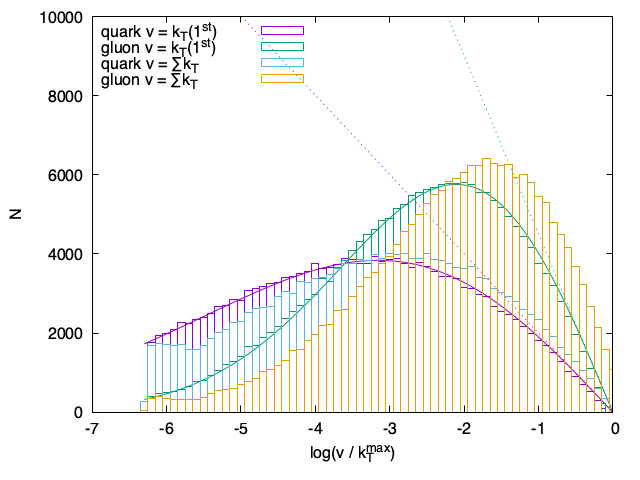
\includegraphics[width=.9\linewidth]{plotKT.png}
\end{center}



We can see that the all-order description damps the divergent behaviour of a pure fixed-order prediction for \(k_T\to0\).
We show separately the first emission alone, which can be compared to the analytic expression in Eq. \eqref{eq:Dsud} given by the solid line and is in excellent agreement with the shower.
In addition, we include a dotted line that corresponds to the fixed-order expression that is logarithmically divergent.
Given \(C_A > C_F\), we also see how a gluon generates more emissions than quarks.
This property can be exploited to try and discriminate between ``quark jets'' and ``gluon jets''.


\begin{center}
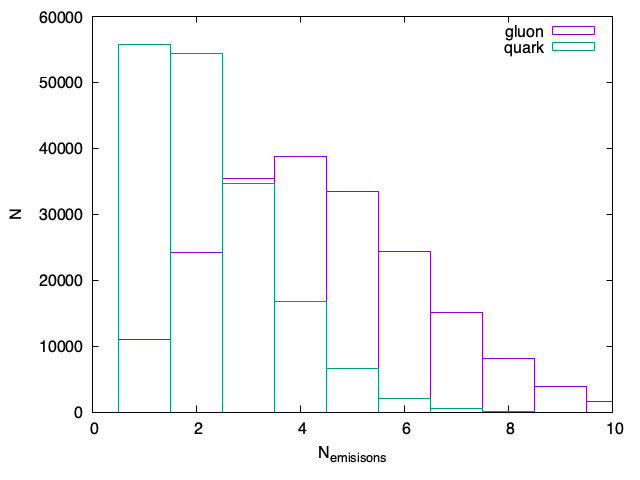
\includegraphics[width=.9\linewidth]{plotN.png}
\end{center}




\begin{quote}
\begin{itemize}
\item To increase the amount of emissions, try out setting the strong coupling to \(\alpha_s=0.5\).
How does the picture change?
\end{itemize}
\end{quote}
\end{document}